\documentclass[10pt,a4paper]{article}
\usepackage[T1]{fontenc}
\usepackage[utf8]{inputenc}
\usepackage{lmodern,microtype}
\usepackage[top=17mm,bottom=18mm,left=20mm,right=20mm]{geometry}
\usepackage{amsmath,amssymb,graphicx,booktabs}
\usepackage{xcolor,caption,enumitem,titlesec}
\usepackage[hidelinks]{hyperref}
\hypersetup{pdftitle={Presence-Filtered Self-Training for Instrument Detection and Template Answering with Tool Priors},pdfauthor={Omar Choudhry},pdfsubject={AIMS Lab method report for SurgVU 2026}}
\definecolor{ink}{HTML}{20344A}
\definecolor{muted}{HTML}{546577}
\definecolor{teal}{HTML}{177E89}
\captionsetup{font=small,labelfont=bf,skip=4pt}
\titleformat{\section}{\normalfont\large\bfseries\color{ink}}{\thesection}{0.6em}{}
\titleformat{\subsection}{\normalfont\normalsize\bfseries}{\thesubsection}{0.5em}{}
\titlespacing{\section}{0pt}{8pt}{3pt}
\titlespacing{\subsection}{0pt}{6pt}{2pt}
\setlength{\parskip}{3pt}
\setlength{\parindent}{0pt}
\setlength{\abovedisplayskip}{5pt}
\setlength{\belowdisplayskip}{5pt}
\setlength{\textfloatsep}{8pt}
\setlength{\intextsep}{7pt}
\newcommand{\hdr}{%
\begin{center}
{\Large\bfseries\color{ink} Presence-Filtered Self-Training for Instrument Detection\\[2pt]
and Template Answering with Tool Priors}\\[7pt]
{\normalsize Omar Choudhry}\\[3pt]
{\small Artificial Intelligence in Medicine and Surgery Group, School of Computer Science,\\
University of Leeds, Leeds LS2 9JT, United Kingdom}\\[2pt]
{\small \href{mailto:O.Choudhry@leeds.ac.uk}{O.Choudhry@leeds.ac.uk}\quad
\href{https://orcid.org/0000-0003-4434-3550}{ORCID 0000-0003-4434-3550}}\\[3pt]
{\small\color{muted} Team AIMS Lab\quad$\cdot$\quad Categories 1 and 2}
\end{center}\vspace{-1mm}\noindent\textcolor{teal}{\rule{\linewidth}{0.6pt}}\vspace{1mm}}

\begin{document}
\hdr

\section{Introduction}
We submitted two independent systems for SurgVU 2026. Our Category 1 detector returns instrument
boxes, classes and confidence scores for every video frame. We combine human box annotations with
detector proposals filtered by tool-installation labels to train the clevis-scale detector. Our Category 2
answerer combines the question's grammatical form with instrument frequencies from the training
labels. It generates short declarative answers without reading the video. Figure~\ref{fig:method}
shows both inference paths.

\begin{figure}[ht]
\centering
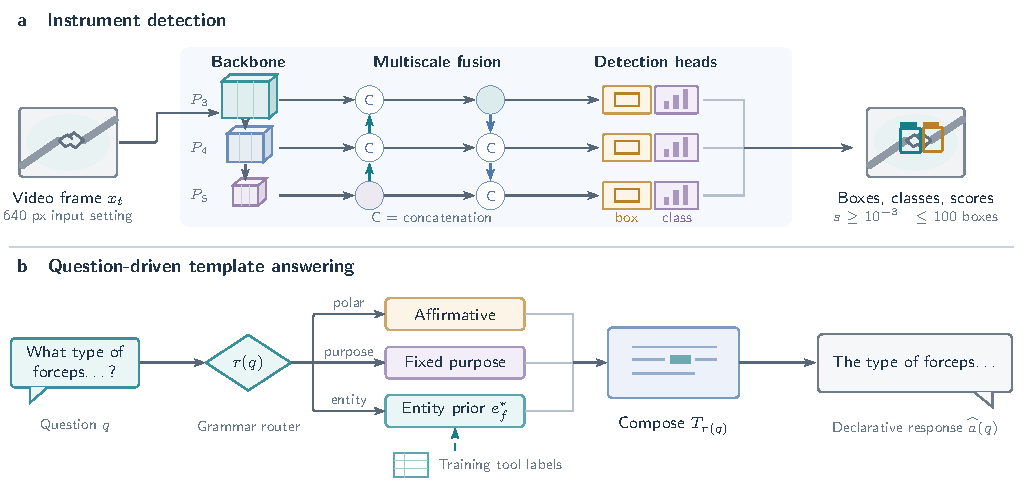
\includegraphics[width=\linewidth]{fig_method.pdf}
\caption{The two inference paths. (a) A framewise YOLO26 detector with multiscale feature fusion. Tensors and instrument frames are schematic. (b) Grammar routes a question
to an affirmative polarity, a fixed purpose phrase or an entity prior, then a template composes
the response.}
\label{fig:method}
\end{figure}

\section{Category 1}
\textbf{Detector and inference.}
We initialise a medium YOLO26 model~\cite{yolo26} from pretrained weights.
At inference, the container loads the selected detector checkpoint and processes every decoded frame
independently. With input-size setting 640 pixels, the wrapper retains at most 100 detections above confidence
$10^{-3}$. For candidate predictions $f_\theta(x_t)$, the output is
\begin{equation}
\widehat{\mathcal D}_t = \operatorname{Top}_{100}
\bigl\{(b,c,s)\in f_\theta(x_t)\mid s\geq 10^{-3}\bigr\},
\label{eq:detect}
\end{equation}
where $b$ is a box, $c\in\{1,\ldots,14\}$ is the instrument class and $s$ is its confidence.
The wrapper writes four box corners in the original frame coordinates, with the class and frame
index. Inference uses no temporal smoothing or ensemble.

\textbf{Supervision and training.}
Human COCO annotations supply the target boxes. We use videos 1--5 for local training and videos
6--7 for validation. Following early experiments with Grad-CAM proposals~\cite{gradcam}, we use a
detector trained on human boxes to generate additional labels. A proposal $(b,c,s)$ is retained only
when its confidence passes $\tau$ and class $c$ is installed at that time
\begin{equation}
\widetilde{\mathcal D}^{\mathrm{filter}}_t =
\bigl\{(b,c)\mid (b,c,s)\in f_\phi(x_t),\ s\geq\tau,\ c\in I_t\bigr\},
\qquad \tau=0.25,
\label{eq:filter}
\end{equation}
where $I_t$ is the installed-tool set. We retrain on the retained pseudo-labels and human-labelled
frames with seeds 0, 1 and 2, then select the seed-2 checkpoint by local validation mAP.
The proposer excludes the held-out videos and uses its last checkpoint. Installation constrains
the class label but does not establish visibility.

\section{Category 2}
\textbf{Question routing and answer composition.}
A leading auxiliary routes a question to the polar branch. Otherwise, ``purpose'' or an initial
``why'' selects the purpose branch. All remaining questions use the entity branch. The response is
\begin{equation}
\widehat a(q)=T_{r(q)}\bigl(q,z(q)\bigr),\qquad
z(q)=\begin{cases}
\mathrm{True} & r(q)=\mathrm{polar},\\
\text{``to grasp and hold tissue''} & r(q)=\mathrm{purpose},\\
e(q) & r(q)=\mathrm{entity}.
\end{cases}
\label{eq:answer}
\end{equation}
Here $r$ is the router and $T$ the sentence template. Polar answers are always affirmative.
Templates reuse the question's wording in declarative order without enforcing a fixed word count.

\textbf{Instrument prior.}
The prior uses \texttt{tools.csv} and deduplicated task segments in \texttt{tasks.csv}
across 155 training cases, yielding $N=1{,}850$ segments. A tool belongs to segment $j$ when its installation interval overlaps
that segment. Let $S_j$ be this tool set and $\mathcal V_f$ the commercial tool names matching
instrument family $f$. The selected entity is
\begin{equation}
e_f^*=\underset{u\in\mathcal V_f}{\arg\max}\;\frac{1}{N}
\sum_{j=1}^{N}\mathbf 1\{u\in S_j\}.
\label{eq:prior}
\end{equation}
The longest matching family name in the question selects $f$. Organ and procedure questions use
fixed phrases. Unmatched entity questions fall back to ``the tissue''. The visual task classifier is disabled. The active path loads no neural model and opens no video.

\textbf{Evaluation and interpretation.}
The organiser's evaluator ranks BERTScore-F1~\cite{bertscore}, using \texttt{roberta-large}
with baseline rescaling. For each question it takes the maximum over the reference answers, then
averages across questions. Our diagnostic scripts probe constant answers, polarity and sentence length on 11 public examples.
These probes do not establish visual understanding. The fixed affirmative branch and entity prior
cannot verify events in an unseen clip.

\section{Availability}
The implementation is available at \url{https://github.com/omariosc/surgvu-aims}
under the MIT licence, with public source release \texttt{e644608}.
Challenge data and third-party software remain subject to their own terms.

{\small
\bibliographystyle{unsrt}
\bibliography{references}
}
\end{document}
